
  
\documentclass{exam}
\usepackage[utf8]{inputenc}
\usepackage{upgreek}
\usepackage[margin=1in]{geometry}
\usepackage{amsmath,amssymb}
\usepackage{multicol}
\usepackage{stmaryrd}
\usepackage{graphicx}
\usepackage{caption}
\usepackage{tikz}
\usepackage{dsfont}
\usepackage{enumitem}
\usepackage{hyperref}
\usetikzlibrary{matrix}
\newcommand\tab[1][1cm]{\hspace*{#1}}
\pagestyle{head}
\firstpageheader{}{}{}
\runningheader{\examnum}{\class}{\name}
\runningheadrule
\newcommand{\class}{Fundamentos de bases de datos}
\newcommand{\term}{Facultad de Ciencias UNAM}
\newcommand{\examnum}{Practica 01 - Bitácora}
\newcommand{\examdate}{07/03/2022}
\newcommand{\name}{Sela Farrera Ortega - 311617670}
\begin{document}

\noindent
\begin{tabular*}{\textwidth}{l @{\extracolsep{\fill}} r @{\extracolsep{6pt}} l}
\textbf{\class} & \textbf{\term}\\
\textbf{\examnum} & \textbf{\name}\\
\textbf{\examdate}
\end{tabular*}\\
\rule[2ex]{\textwidth}{2pt}

\section*{Bitácora}

\subsection*{Sistema operativo y versión}

%Aquí describes tu sistema operativo y su versión.
Memoria RAM: 16GB\\
Procesador: Intel Core i7-7700 @ 3.60 GHz\\
Sistema Operativo: Linux\\
KDE Plasma Version: 5.22.5\\
Kernel Version: 5.16.11-100.fc34.x86\_64\\
Arquitectura: 64-bit

\subsection*{Distribución}

%Solamente en el caso de Linux, borra la subsection si tienes windows/mac
Distribución: Fedora release 34

\subsection*{Versión de la instalación}

PostgreSQL 12.10 on x86\_64-pc-linux-gnu, compiled by gcc (GCC) 11.2.1 20220127 (Red Hat 11.2.1-9), 64-bit

\subsection*{Tiempo requerido}

20 min

\subsection*{Explicación del paso a paso}

%Agrega imagenes (no olvides incluirlas en el git)
\begin{enumerate}
	\item Agregar el repositorio remoto de Yum al sistema dnf de Fedora usando el comando:
	
	\verb|$ sudo dnf install https://download.postgresql.org/pub/repos/yum/reporpms/F-31-|
	
	\verb|x86_64/pgdg-fedora-repo-latest.noarch.rpm|

	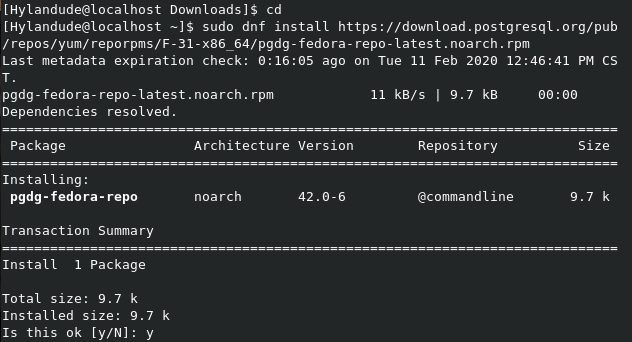
\includegraphics[scale=0.75]{./imgFarrera/postgress_install_1.png}	

	Introduce la contraseña de root (si es requerido) y cuando se solicite acepta la instalación escribiendo 'y'.
	
	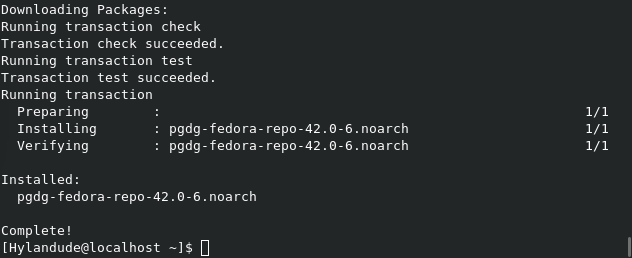
\includegraphics[scale=0.75]{./imgFarrera/postgress_install_2.png}

	\item Instalar PostgreSQL al sistema mediante el siguiente comando:
	
	\verb|$ sudo dnf install postgresql12-server postgresql12|
	
	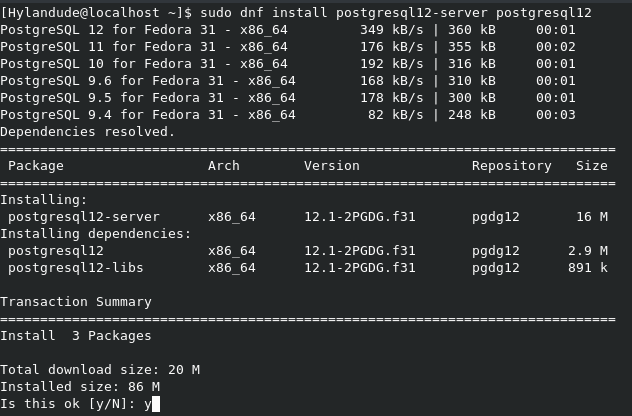
\includegraphics[scale=0.75]{./imgFarrera/postgress_install_3.png}	
	
	Introduce la contraseña de root (si es requerido) y cuando se solicite acepta la instalación escribiendo 'y'.
	
	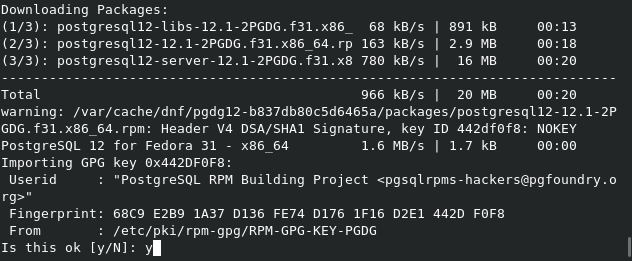
\includegraphics[scale=0.75]{./imgFarrera/postgress_install_4.png}	
	
	Es posible que se te solicite una GPG key esta se debió haber registrado durante el paso anterior. Simplemente acepta escribiendo 'y'
	
	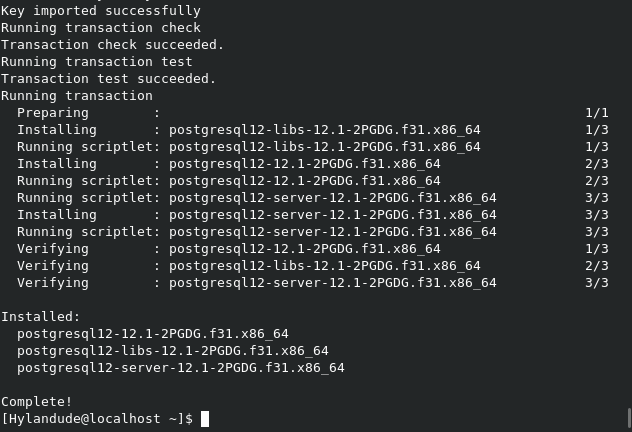
\includegraphics[scale=0.75]{./imgFarrera/postgress_install_5.png}	
	
	\item PostgreSQL ya se encuentra instalado, es necesario incializar el servicio.
	
	\verb|$ sudo /usr/pgsql-12/bin/postgresql-12-setup initdb|
	
	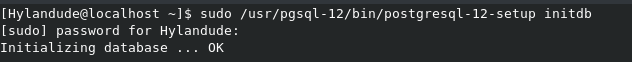
\includegraphics[scale=0.75]{./imgFarrera/postgress_install_6.png}	
	
	Configurar para que se inicie el servicio al prender la computadora.	
	
	\verb|$ sudo systemctl enable --now postgresql-12|
	
	Verificar que este corriendo correctamente
	
	\verb|$ systemctl status postgresql-12|
	
	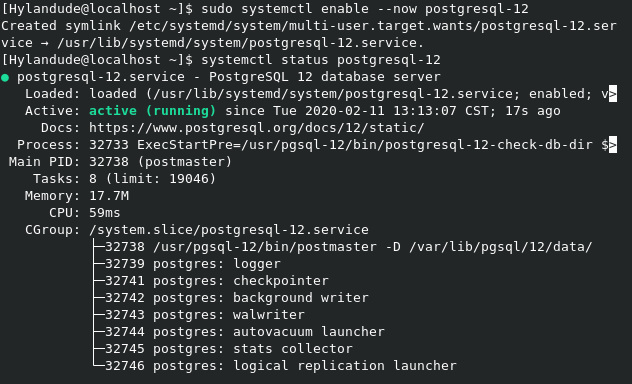
\includegraphics[scale=0.75]{./imgFarrera/postgress_install_7.png}		
	
	\item (Opcional) Si se tiene corriendo un servicio de firewall y es necesario permitir conexiones externas hay que autorizar el servicio.
	
	\verb|$ sudo firewall-cmd --add-service=postgresql --permanent|
	
	\verb|$ sudo firewall-cmd --reload|
	
	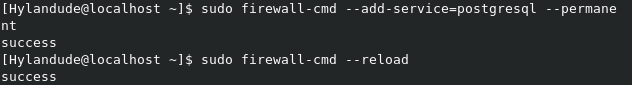
\includegraphics[scale=0.75]{./imgFarrera/postgress_install_8.png}	
	
	\item (Opcional) Si se requieren aceptar conexiones externas hay que agregar las direcciones ip requeridas una por una (o todas como en el ejemplo). Se esta usando emacs como editor en la linea de texto pero se puede remplazar 'emacs -nw' por cualquier otro editor.
	
	\verb|$ sudo emacs -nw /var/lib/pgsql/12/data/postgresql.conf|
	
	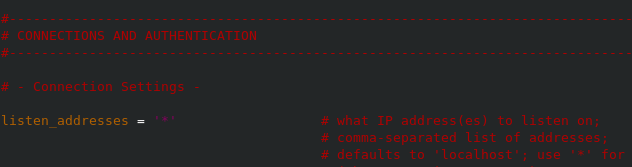
\includegraphics[scale=0.75]{./imgFarrera/postgress_install_9.png}	
	
	Modificar el archivo de configuración con los tipos correctos de autenticación mostrados a continuación.	
	
	\verb|$ sudo emacs -nw /var/lib/pgsql/12/data/pg_hba.conf|
	
	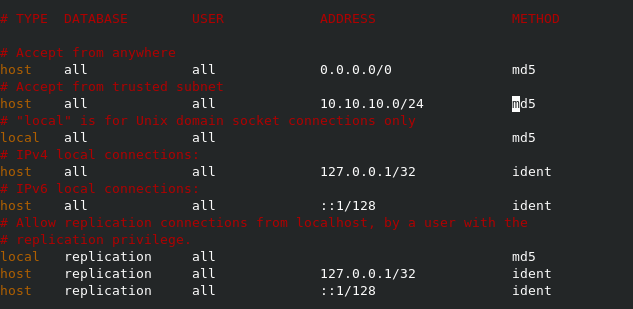
\includegraphics[scale=0.75]{./imgFarrera/postgress_install_10.png}
	
	reiniciar el servicio de PostgreSQL para aplicar los cambios
	
	\verb|$ sudo systemctl restart postgresql-12|
	
	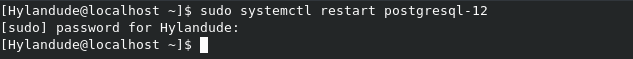
\includegraphics[scale=0.75]{./imgFarrera/postgress_install_11.png}
	
	\item Crear la contraseña para el super usuario de PostgreSQL
	
	\verb|$ sudo su - postgres|
	
	\verb|postgres$ psql -c "alter user postgres with password 'CONTRASEÑA NUEVA'"|
	
	\item (Opcional) Crear un segundo super usuario que no sea root
	
	\verb|postgres$ createuser -P -s -e [NOMBRE DE USUARIO]|	
	
	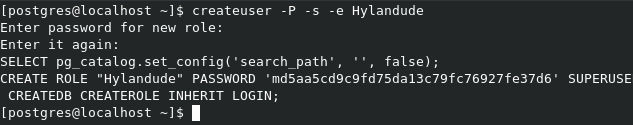
\includegraphics[scale=0.75]{./imgFarrera/postgress_install_12.png}
	
\end{enumerate}

\subsection*{Instalacion de DBeaver}

\begin{enumerate}
	\item Visitar la pagina web https://dbeaver.io/download/ y descargar el paquete RPM
	
	\item En la terminal navegar hacia la carpeta donde fue descargado el archivo y correr el comando
	
	\verb|$ sudo dnf install ./dbeaver-ce-22.0.0-stable.x86_64.rpm|
\end{enumerate}


\subsection*{Comentarios y problemas}

Las capturas de pantalla son de una instalación previa en el mismo sistema pero los pasos se mantienen igual ya que el proceso de instalación no ha cambiado. No hubo ninguna complicación al momento de la instalación.

\begin{thebibliography}{1}
  	\bibitem {}https://computingforgeeks.com/how-to-install-postgresql-12-on-fedora/	
\end{thebibliography}

\end{document}